\chapter{結果}
\label{chap:results}


\begin{figure}[H]
    \centering
    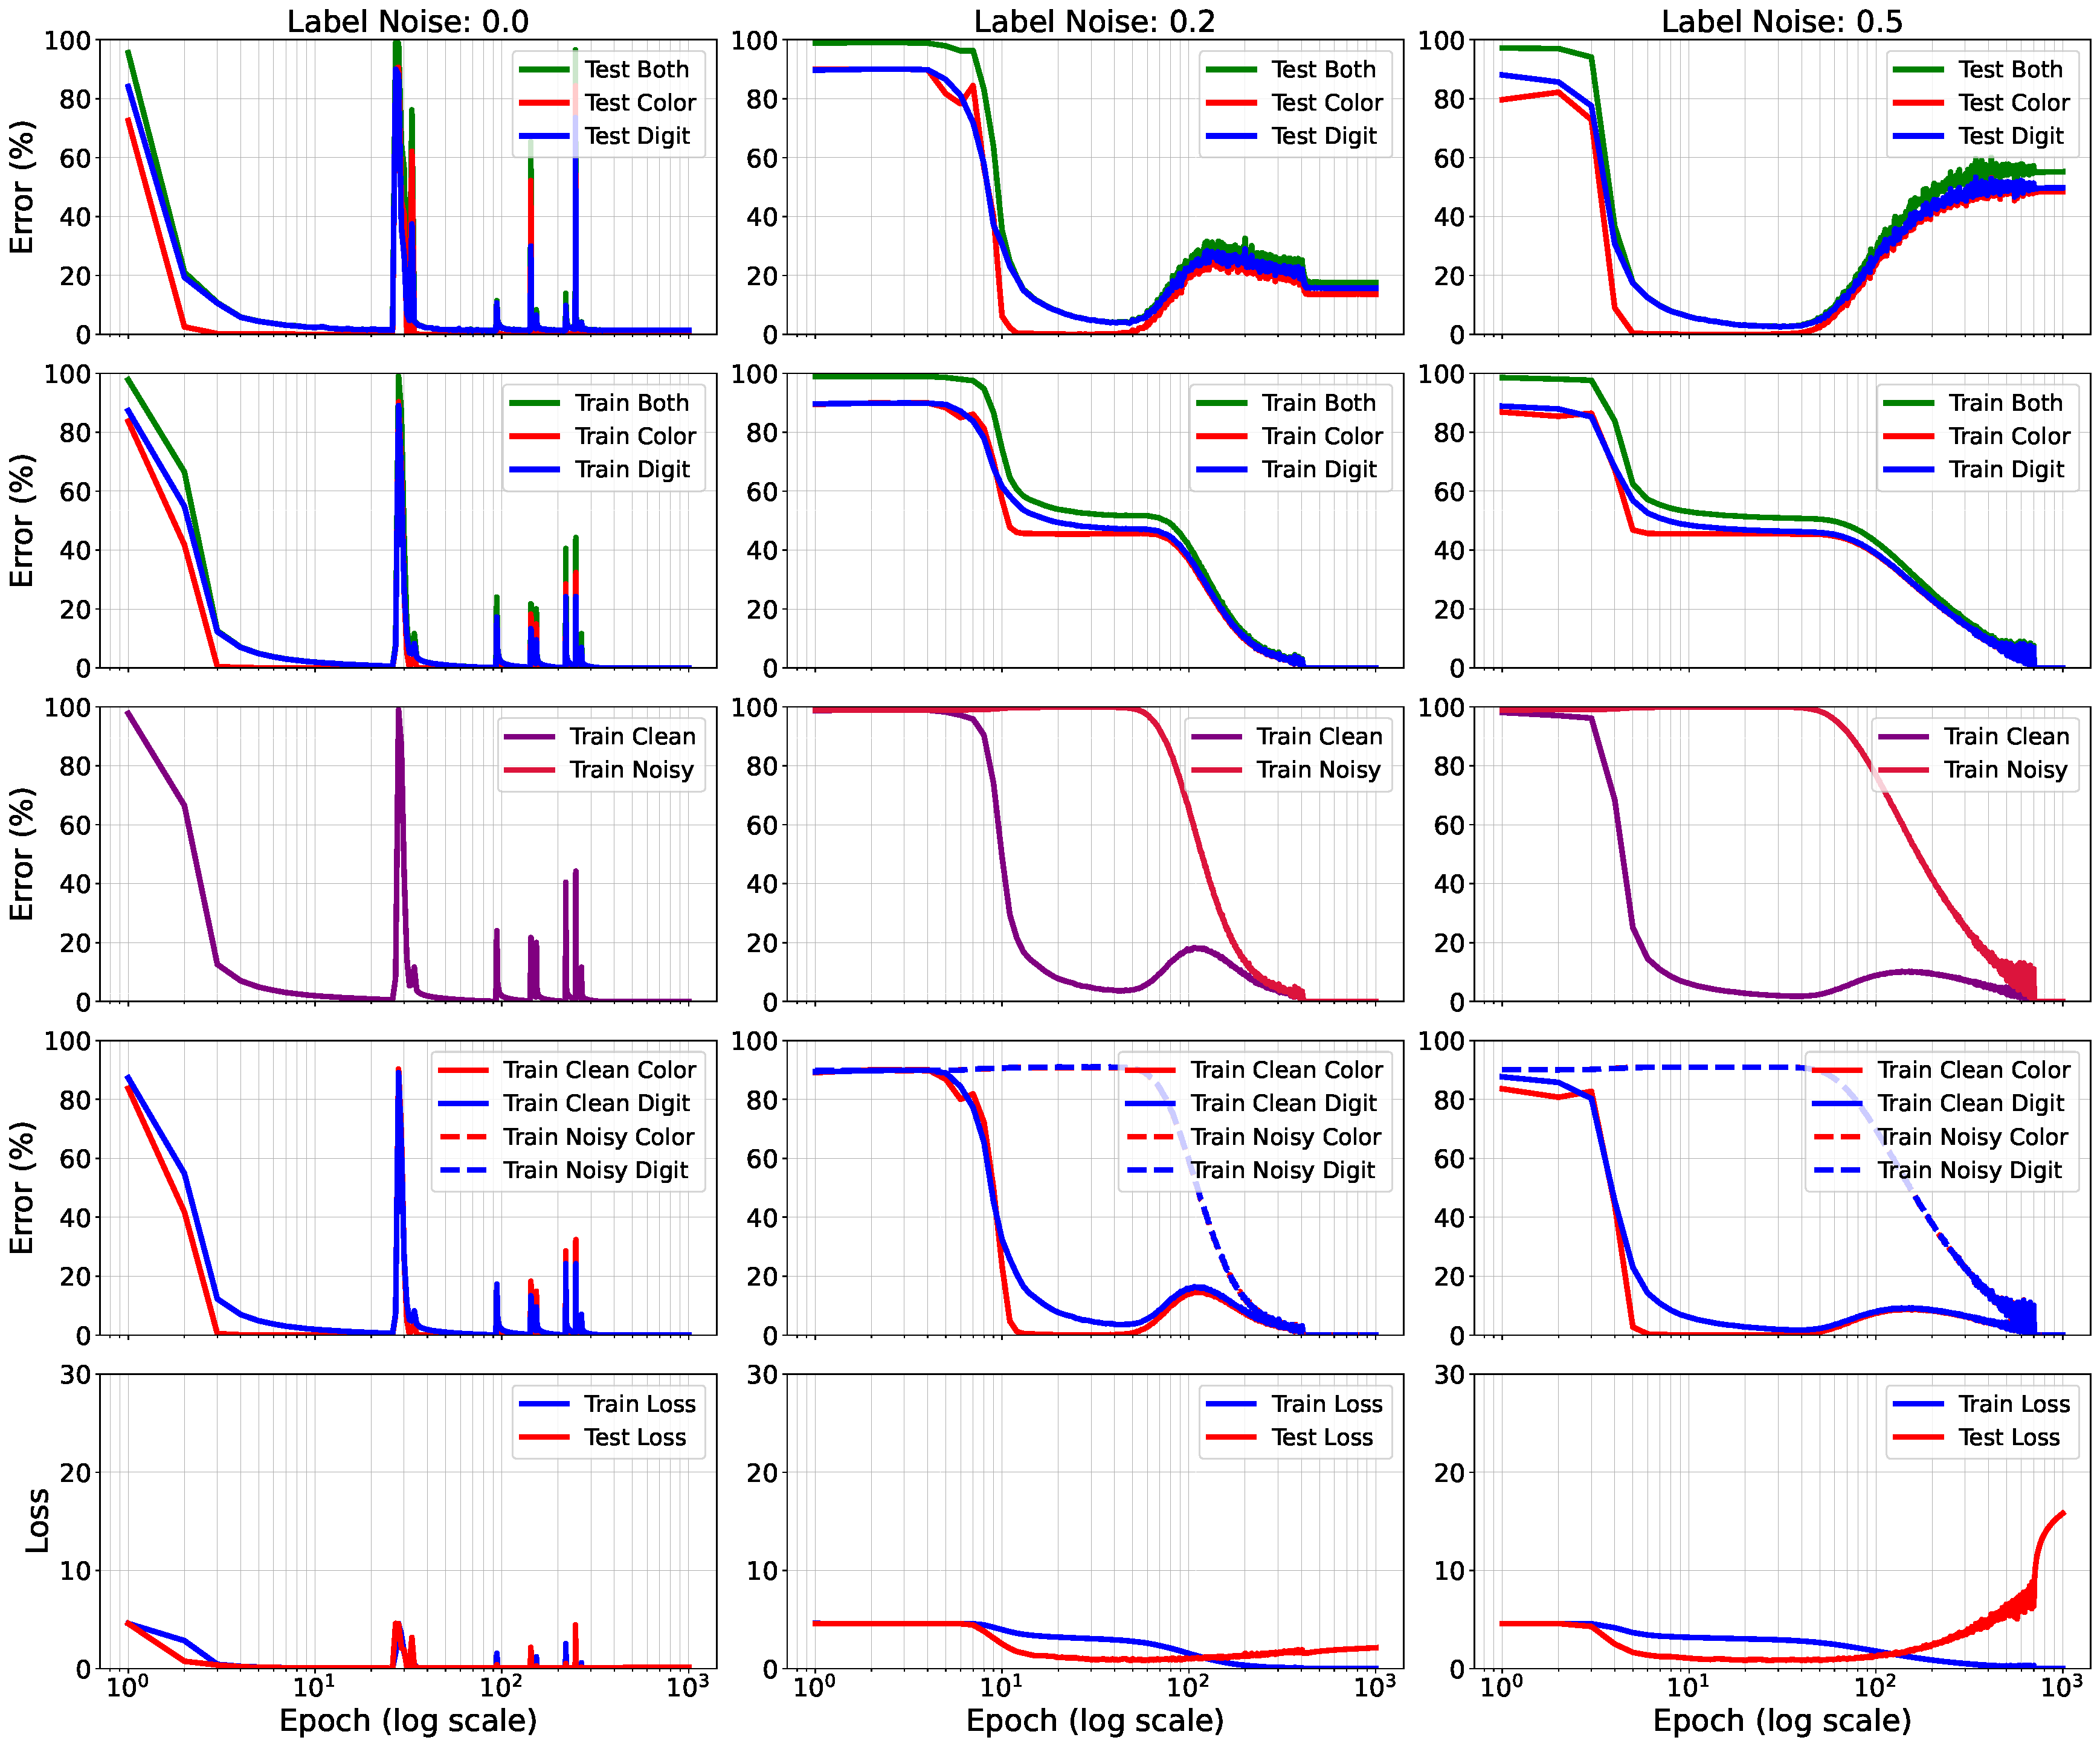
\includegraphics[width=\linewidth]{fig/erroe_metrics_by_variances/error_metrics_by_label_noise_variance_0.pdf}
    \caption{$\sigma^2 = 0$のときのそれぞれのラベルノイズにおける結果}
    \label{fig:errors_by_label_noise_variance_0}
\end{figure}

\begin{figure}
    \centering
    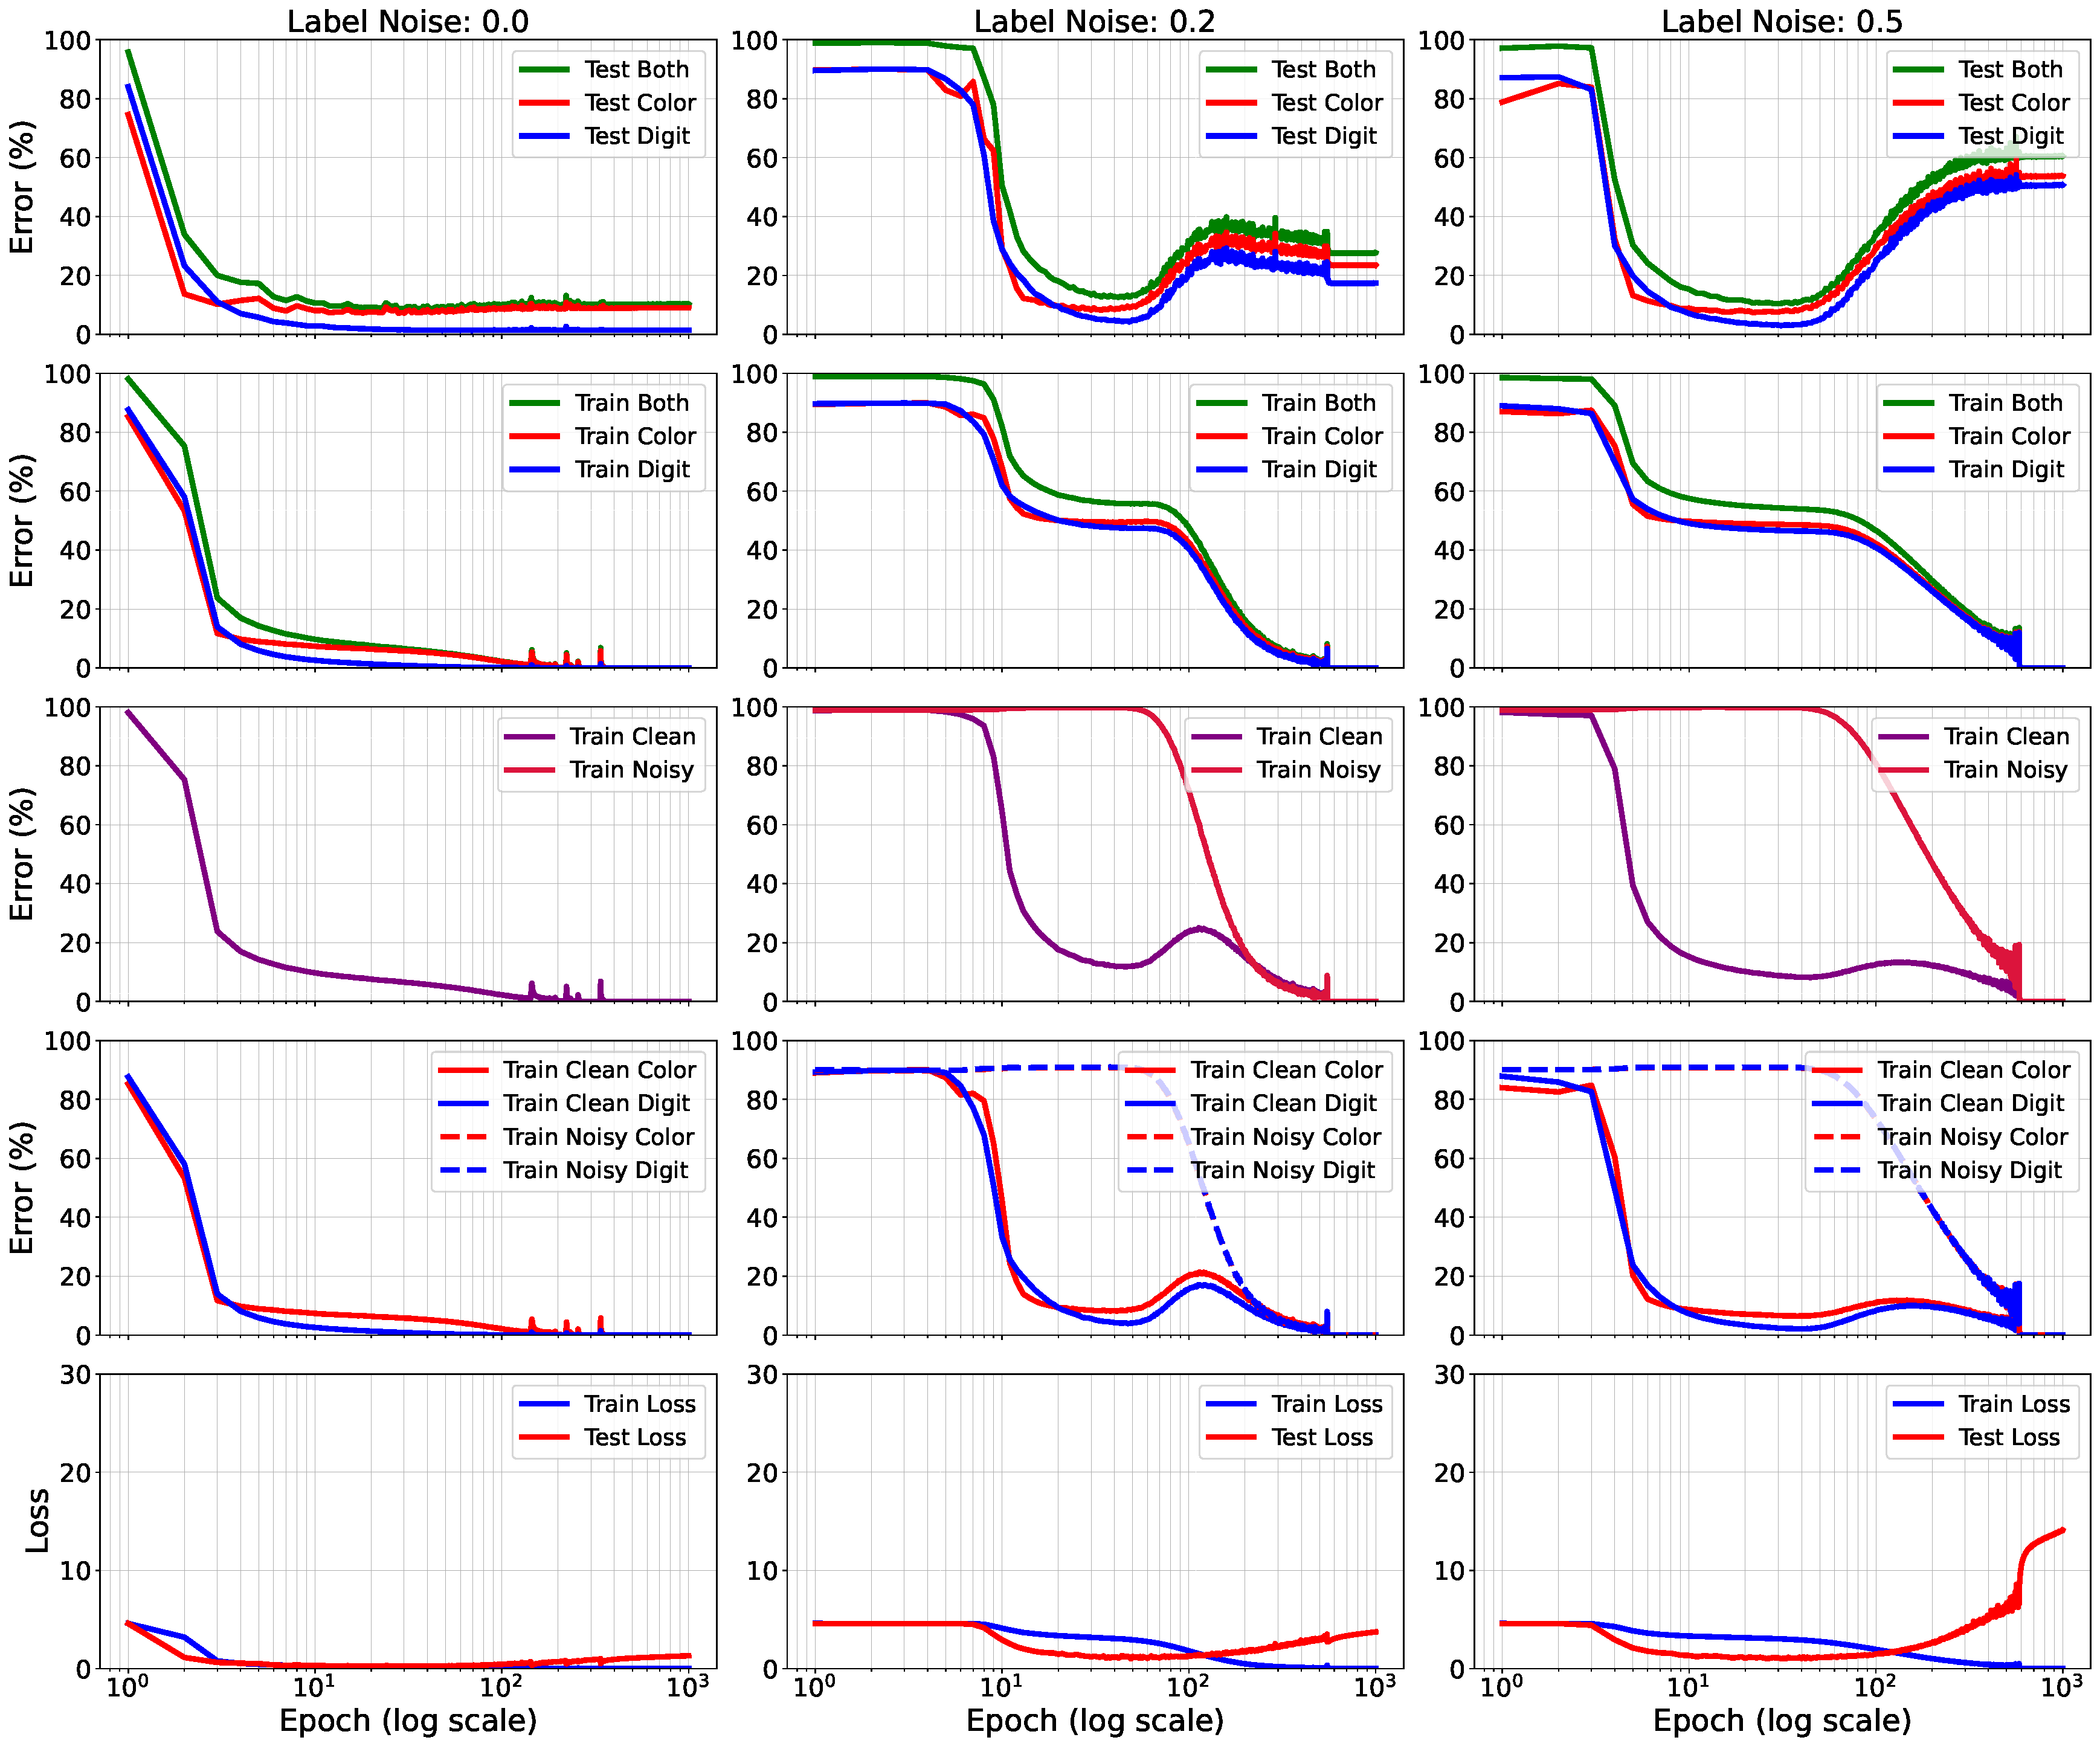
\includegraphics[width=\linewidth]{fig/erroe_metrics_by_variances/error_metrics_by_label_noise_variance_1000.pdf}
    \caption{$\sigma^2 = 10^2$のときのそれぞれのラベルノイズにおける結果}
    \label{fig:errors_by_label_noise_variance_1000}
\end{figure}

\begin{figure}
    \centering
    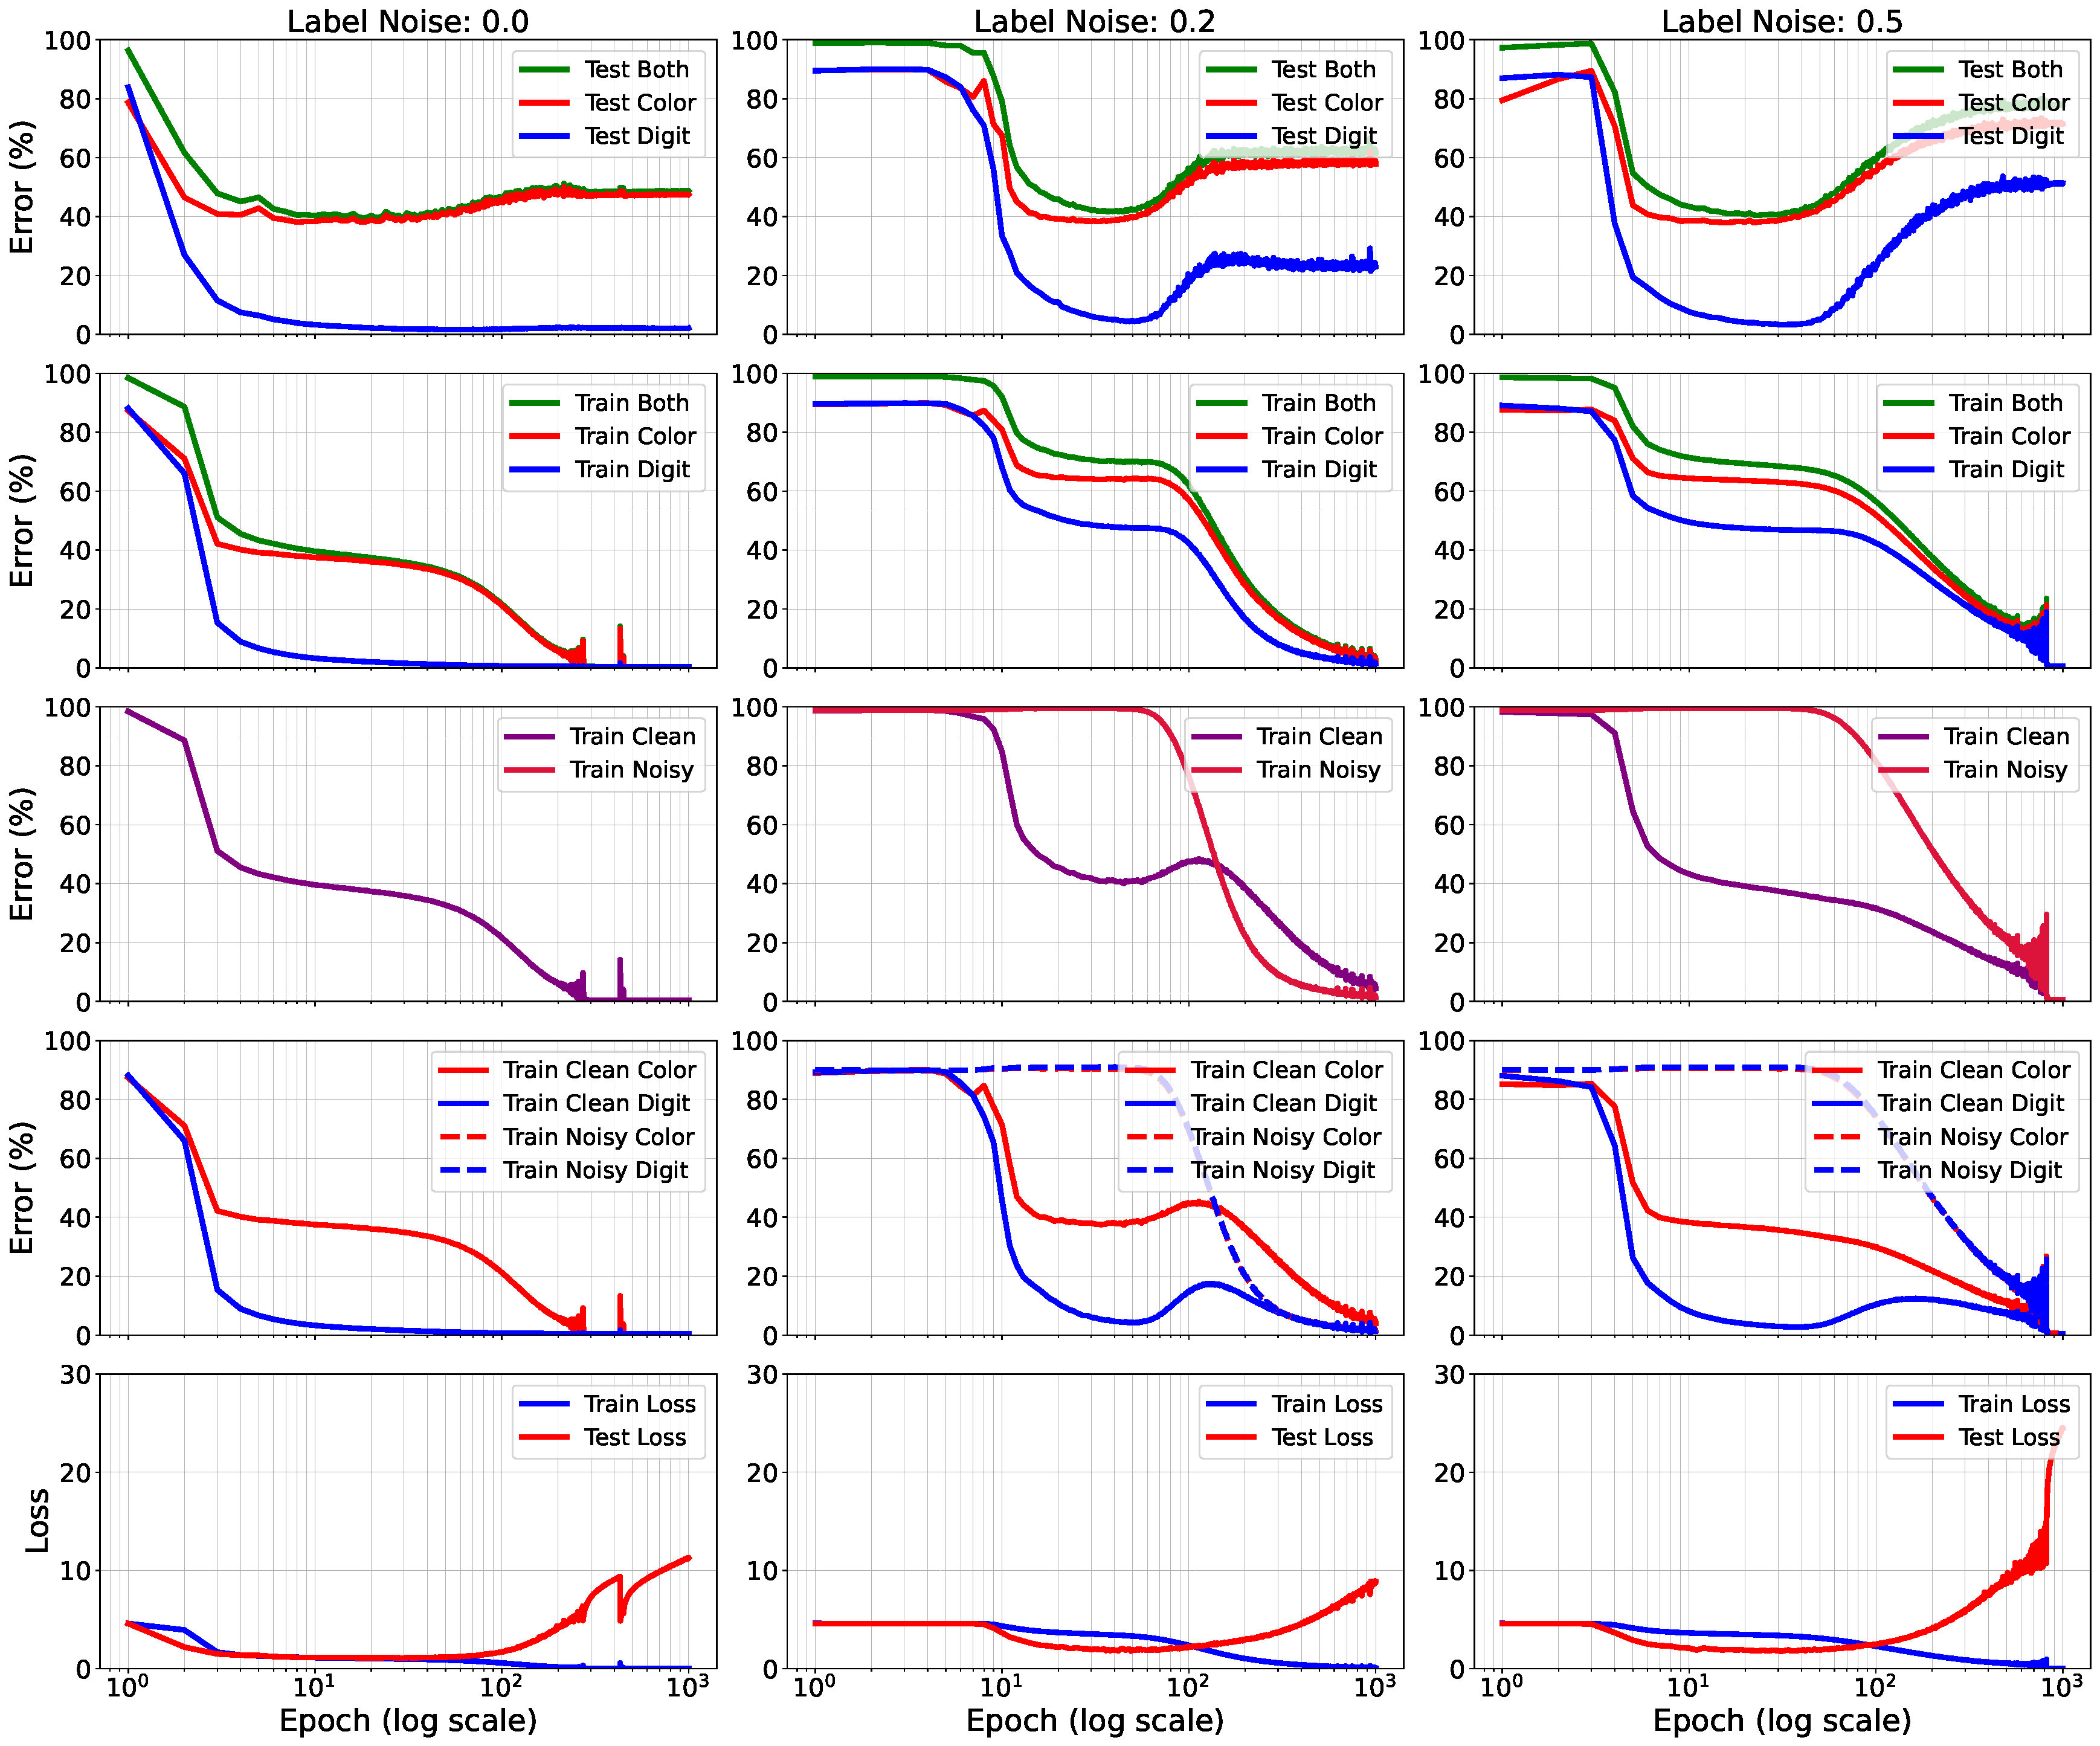
\includegraphics[width=\linewidth]{fig/erroe_metrics_by_variances/error_metrics_by_label_noise_variance_3612.pdf}
    \caption{$\sigma^2 = 10^{3.5}$のときのそれぞれのラベルノイズにおける結果}
    \label{fig:errors_by_label_noise_variance_3612}
\end{figure}

\begin{figure}
    \centering
    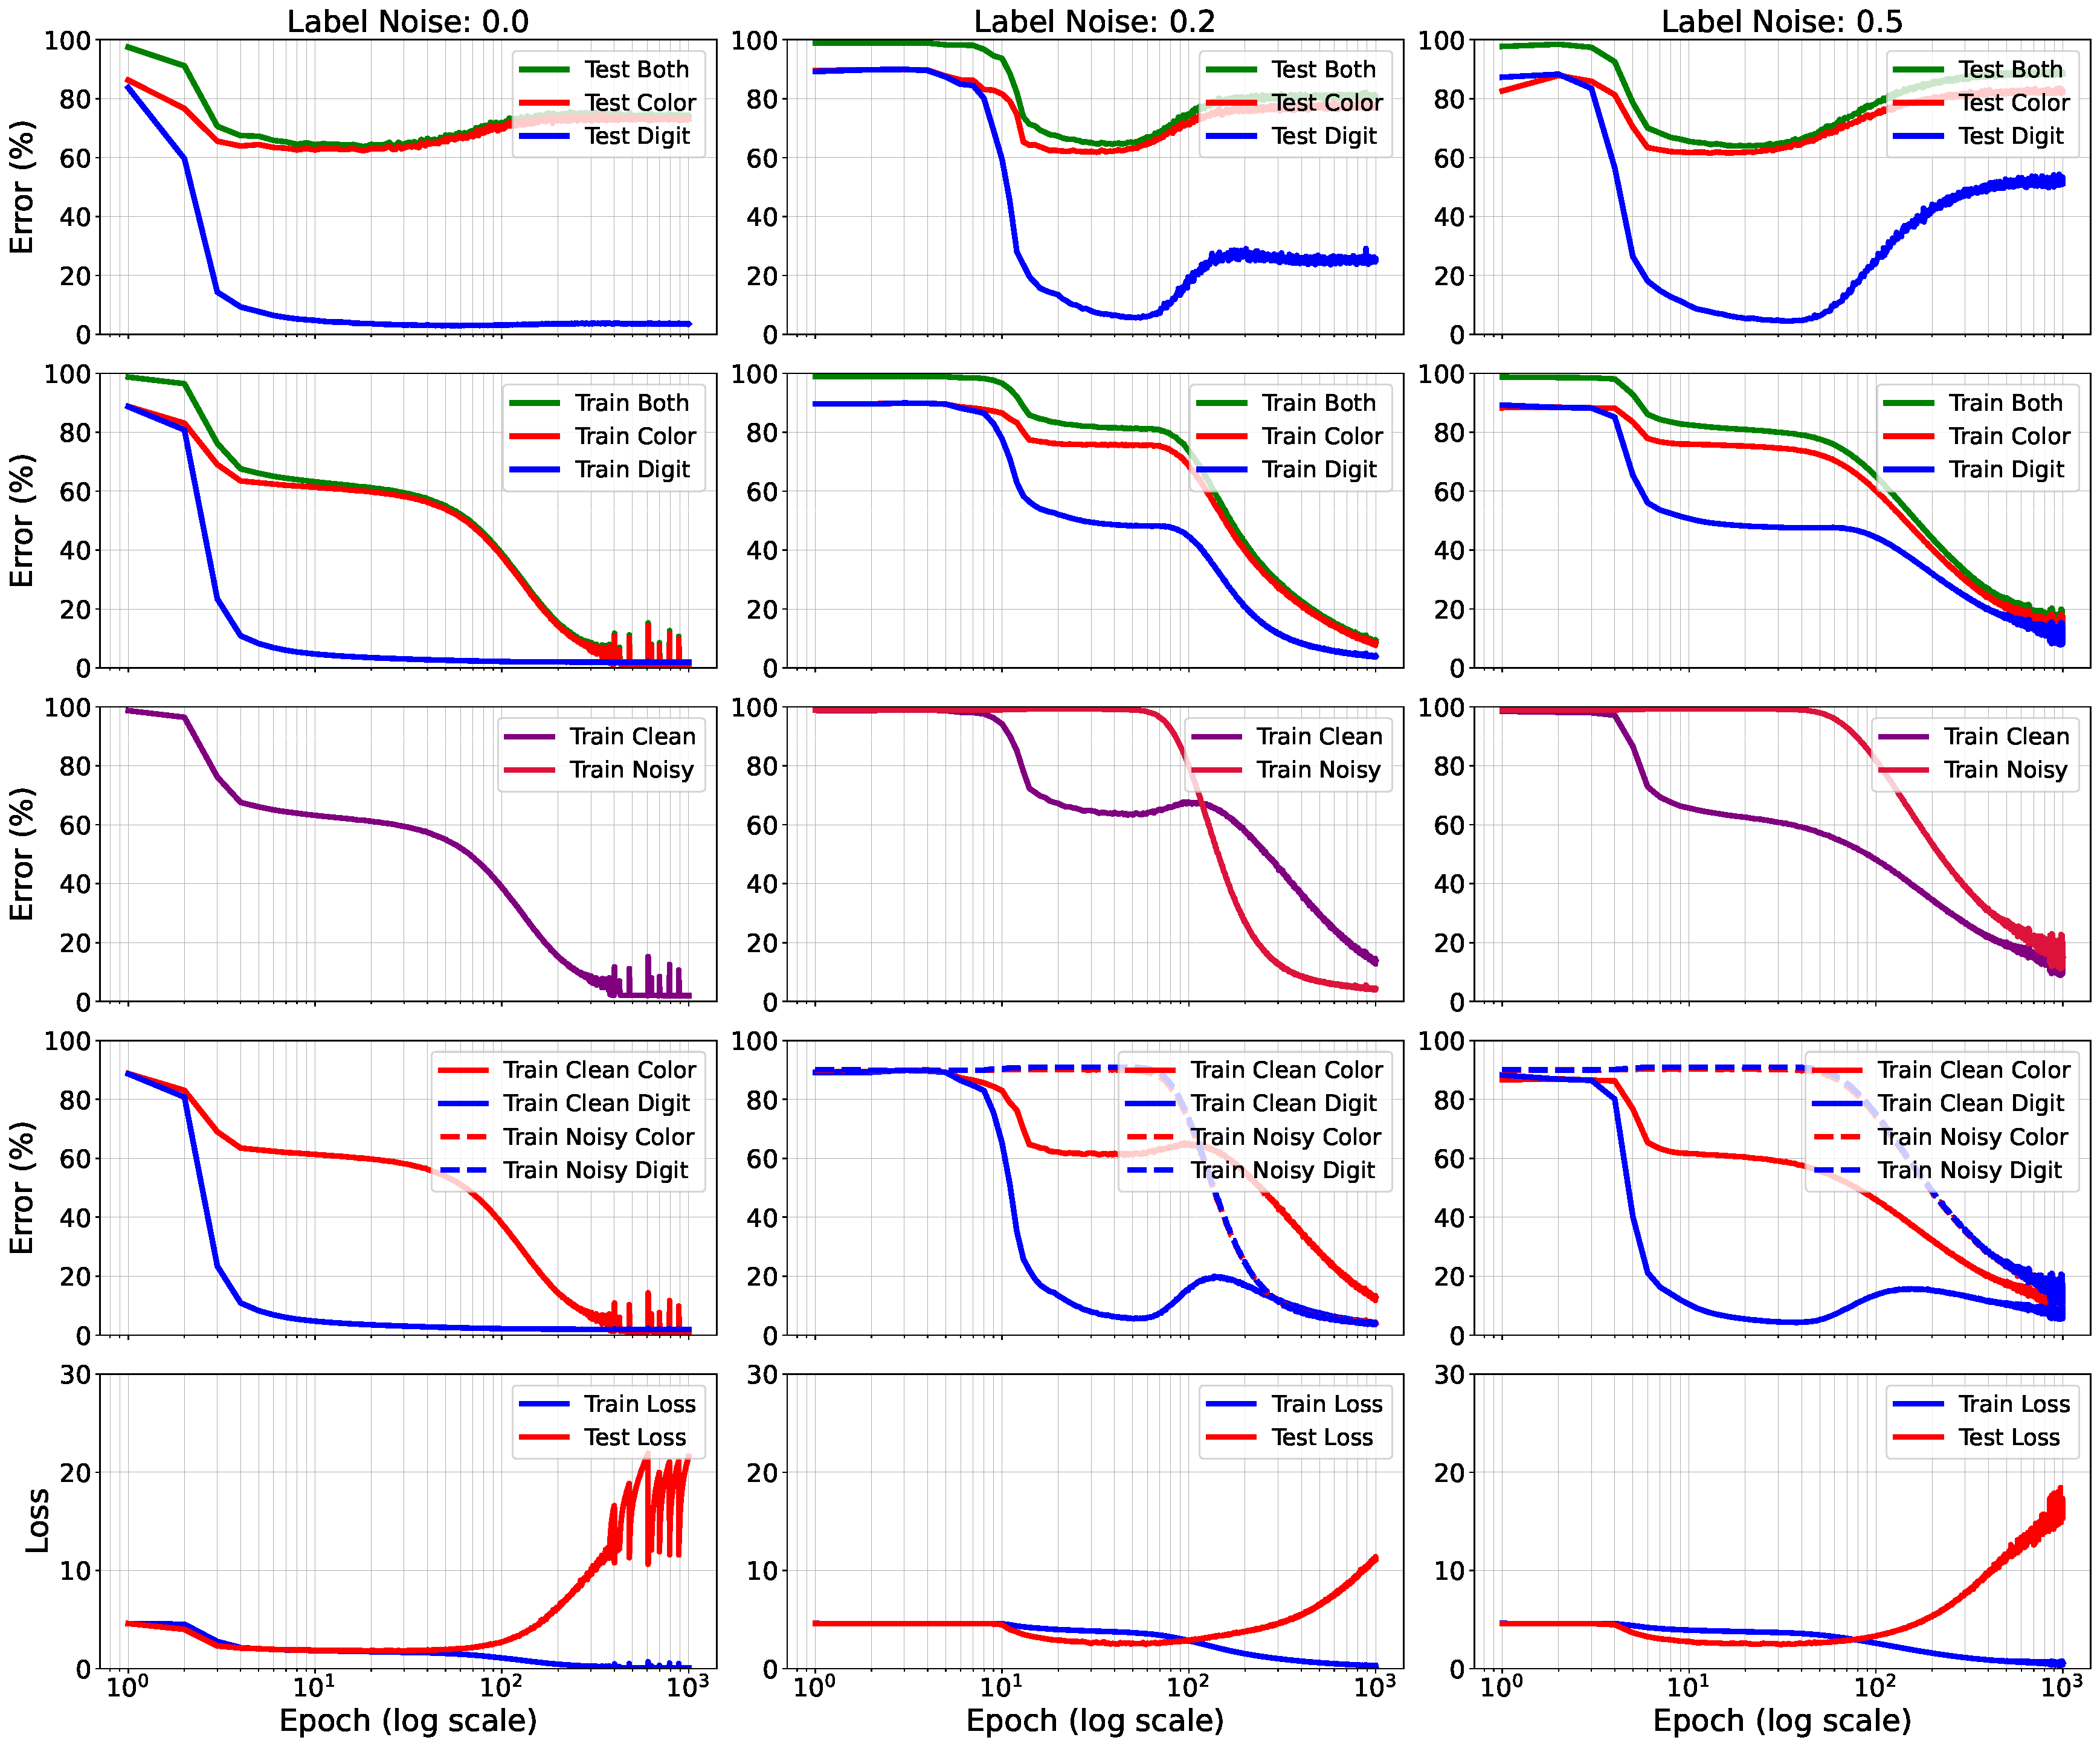
\includegraphics[width=\linewidth]{fig/erroe_metrics_by_variances/error_metrics_by_label_noise_variance_10000.pdf}
    \caption{$\sigma^2 = 10^4$のときのそれぞれのラベルノイズにおける結果}
    \label{fig:errors_by_label_noise_variance_10000}
\end{figure}

\begin{figure}
    \centering
    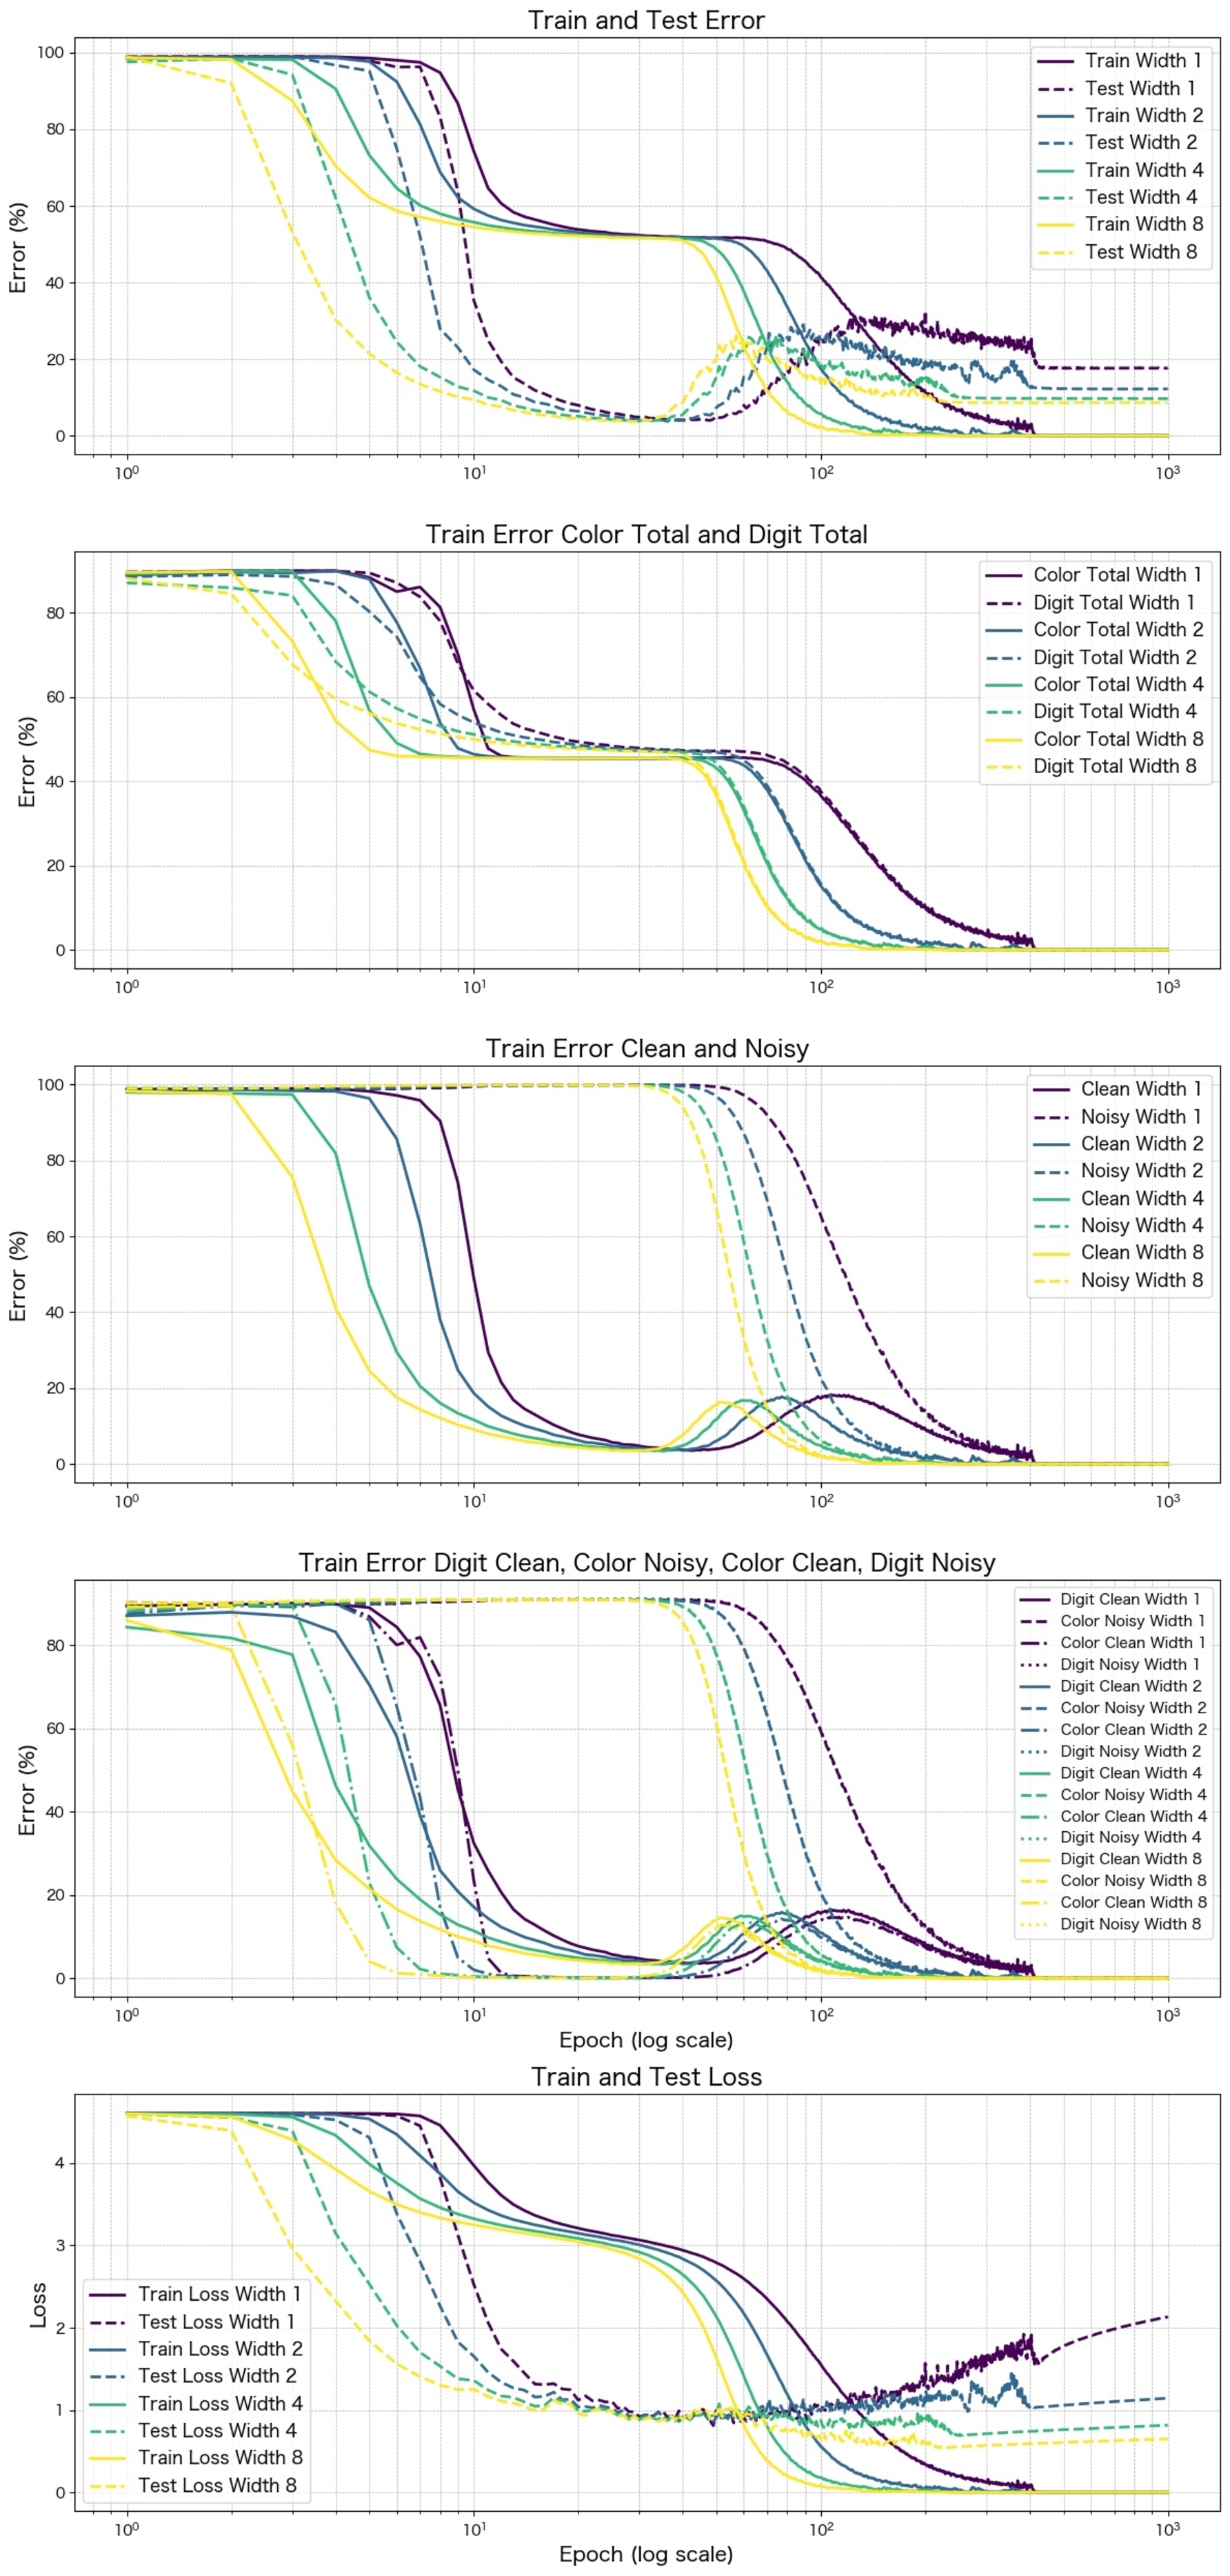
\includegraphics[width=0.7\linewidth]{fig/modelwidth_ln0.2.pdf}
    \caption{$\gamma = 0.2, \sigma^2 = 0$,のときのmodel width別の結果}
    \label{fig:modelwidth_ln02}
\end{figure}

\begin{figure}
    \centering
    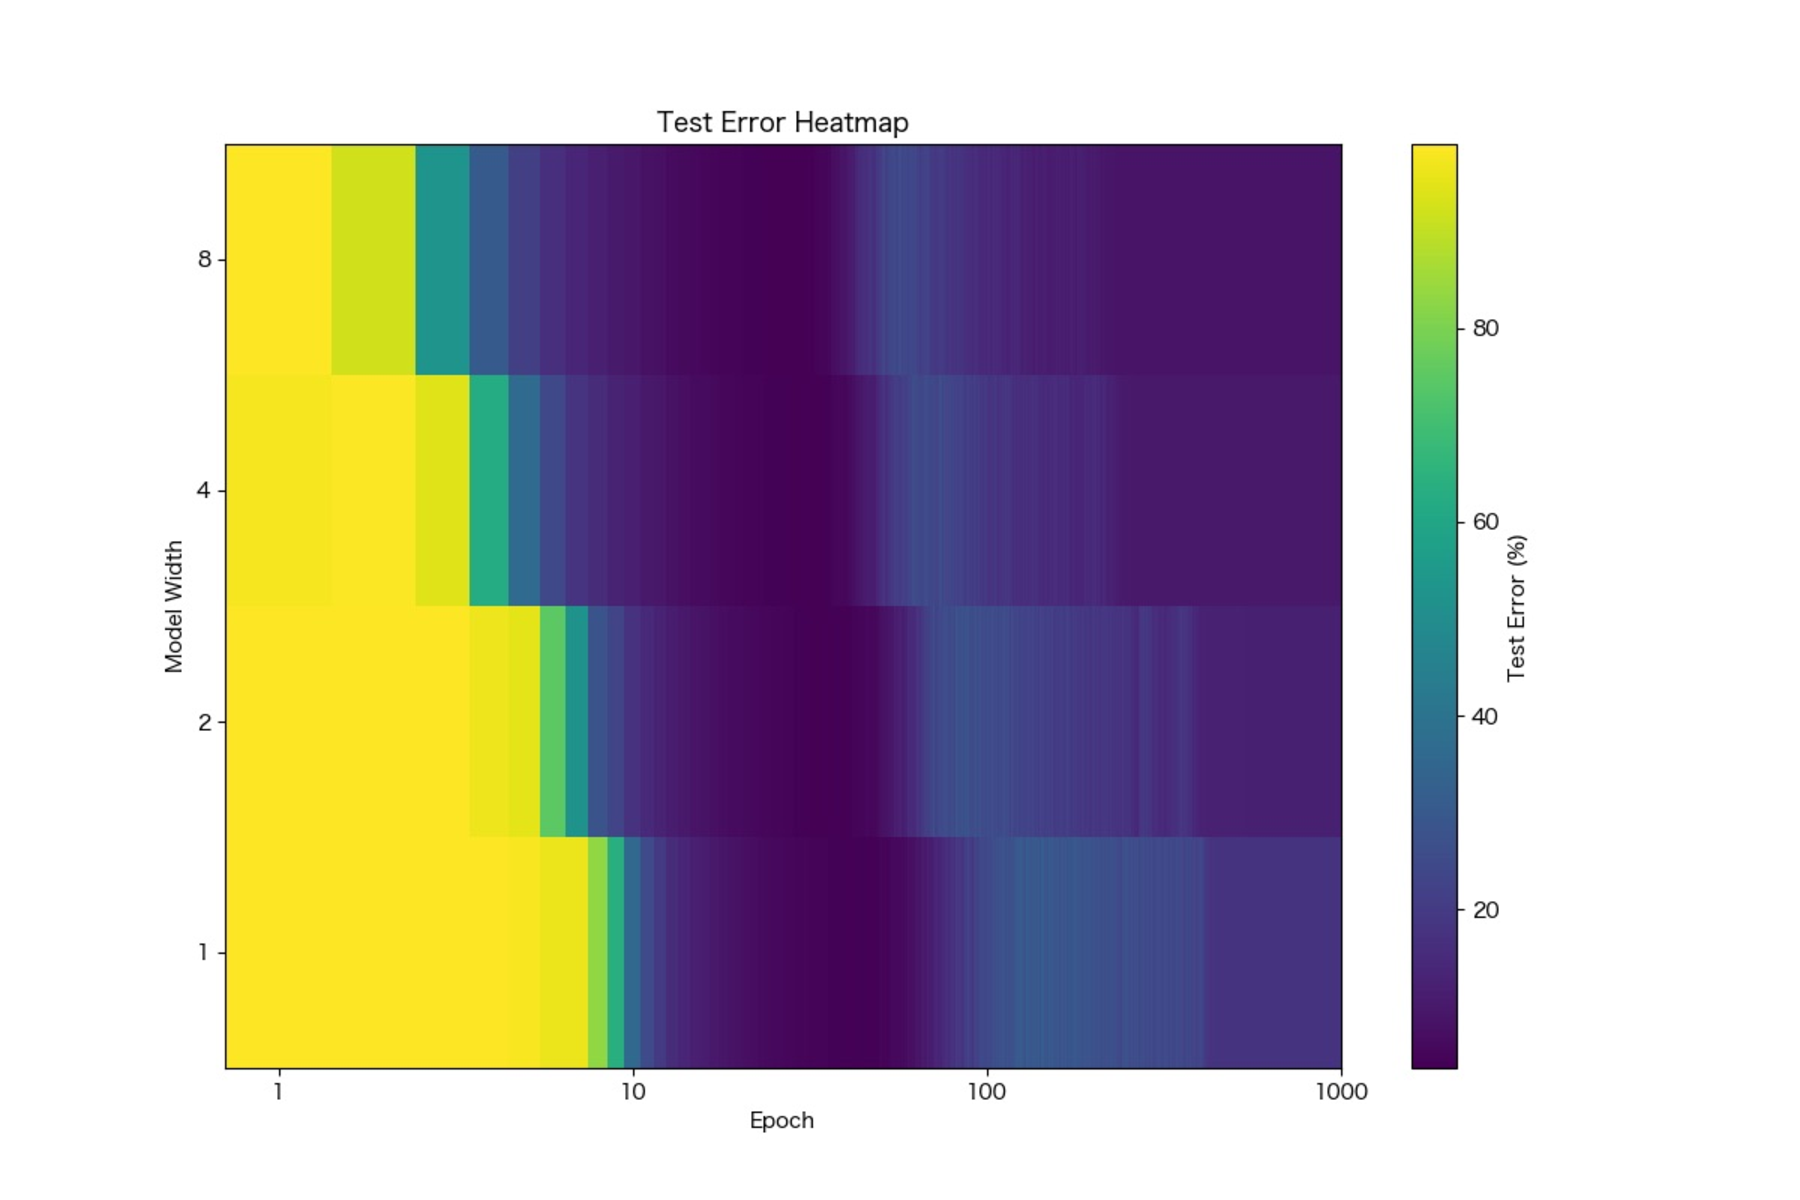
\includegraphics[width=\linewidth]{fig/test_error_heatmap_ln0.2.pdf}
    \caption{$\gamma = 0.2, \sigma^2 = 0$,のときのEpochとModel Widthによるテストエラーのヒートマップ}
    \label{fig:modelwidth_ln1000}
\end{figure}

\begin{figure}
    \centering
    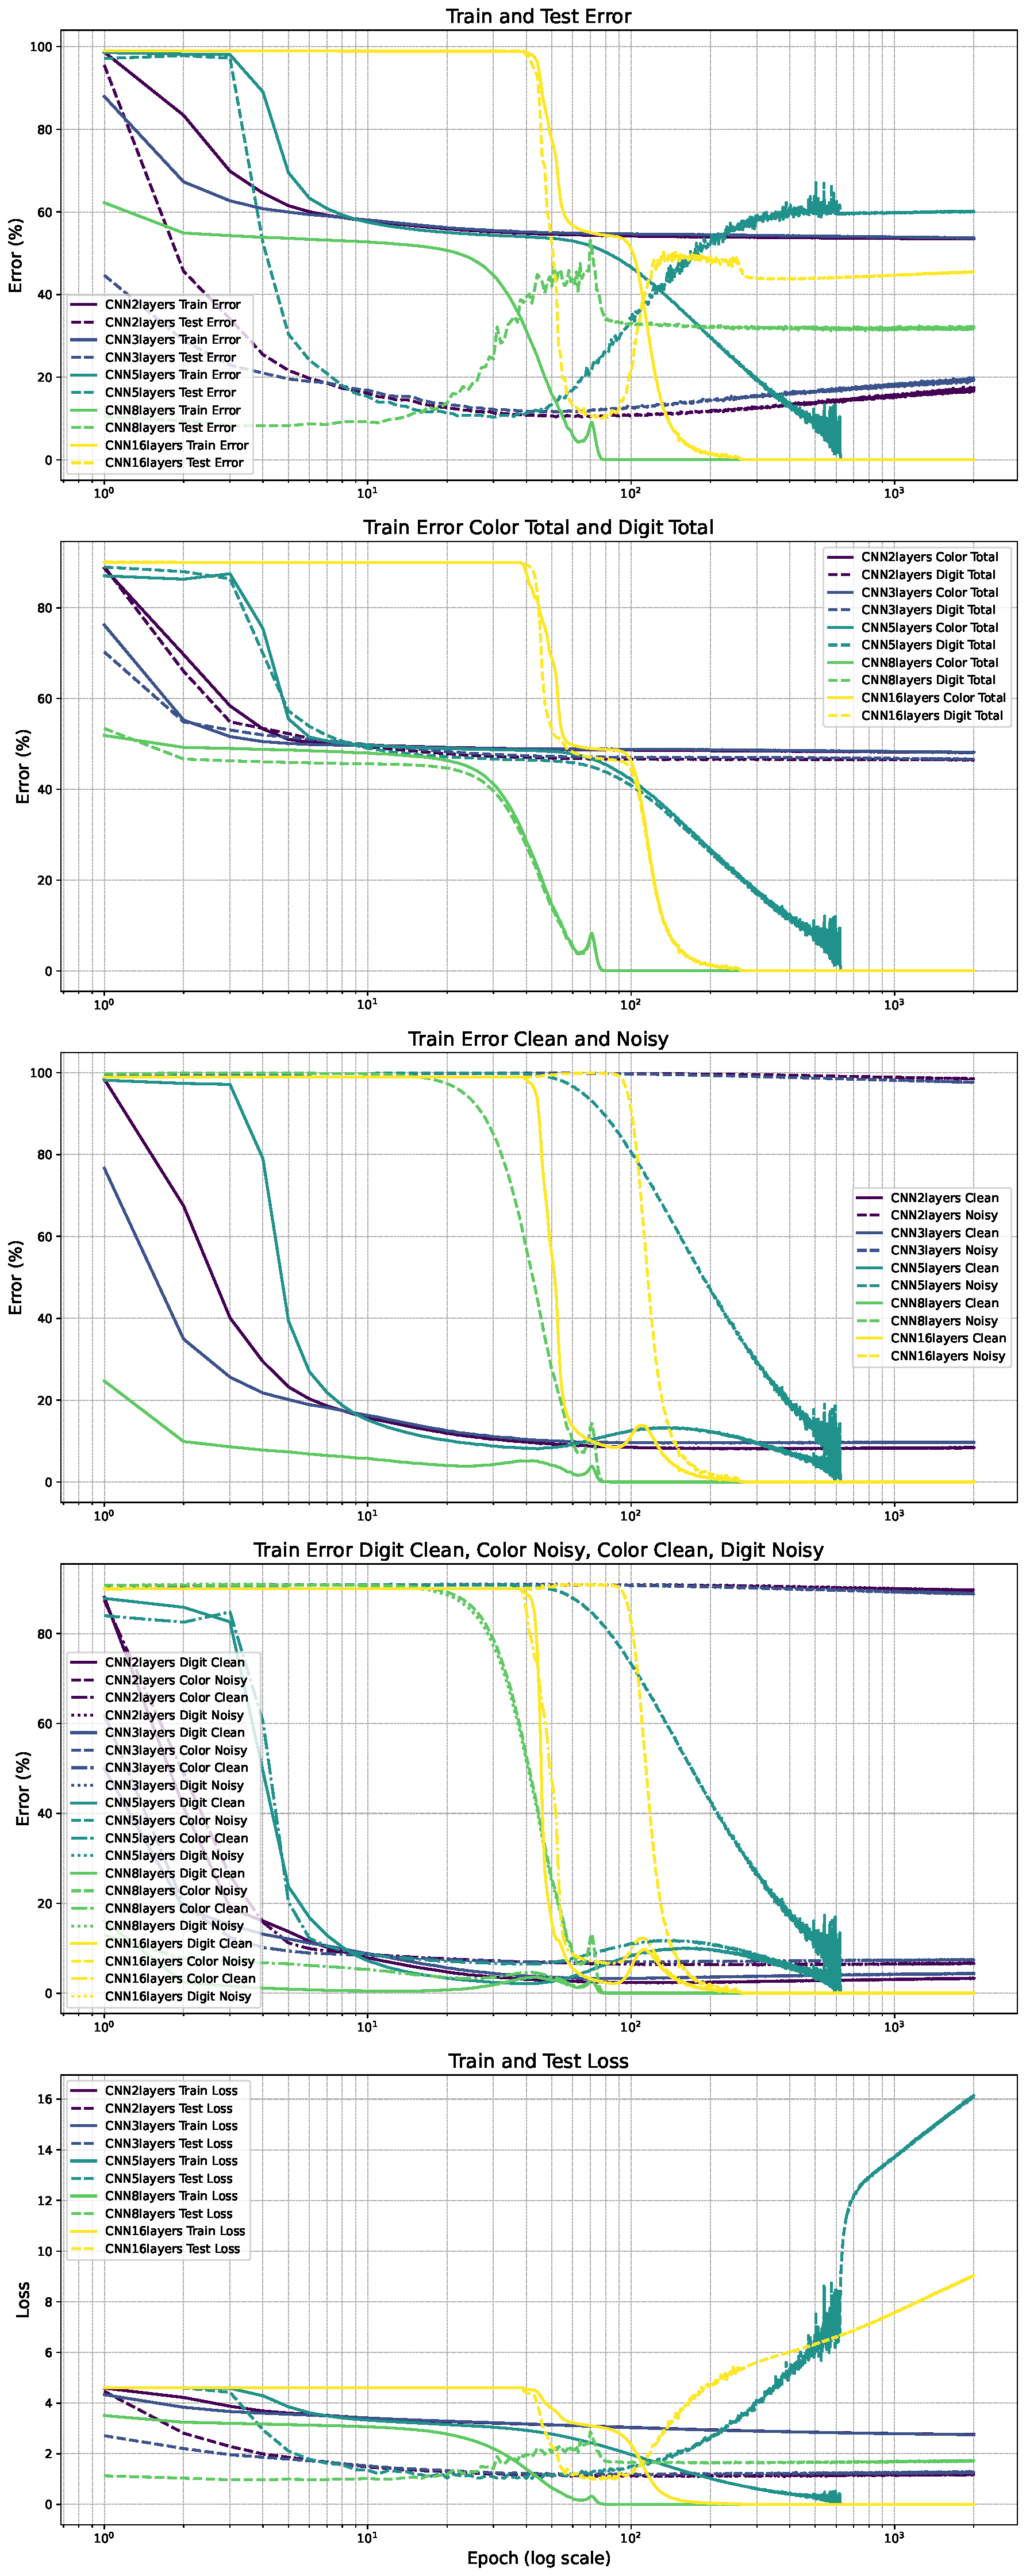
\includegraphics[width=0.5\linewidth]{fig/cnn_layers_comparison.pdf}
    \caption{$\gamma = 0.5, \sigma^2 = 10^3$,のときのCNNの層の深さによる比較}
    \label{fig:cnn_layers_comparison}
\end{figure}
